\thispagestyle{fancy}
\begin{center}
	\LARGE{\textbf{Resistores en paralelo}}
\end{center}
\section{Objetivos}
Al finalizar esta experiencia, usted estará capacitado para:
\begin{enumerate}
	\item 	Medir la corriente en circuito conectados en paralelo
	\item	Usar estos valores para comprobar la ley de las corrientes de Kirchhoff
\end{enumerate}
\section{Conocimientos previos}
La ley de las corrientes de Kirchhoff afirma que la sima algebraica de las corrientes que fluyen hacia un nodo cualquiera de un circuito es igual a cero.
Definiremos las corrientes que fluyen hacia el nodo como positivas, y corrientes que fluyen desde el nodo como negativas. Esto es una simple convención. \\
Para comprobar la ley de las corrientes, mediremos todas las corrientes que circular desde y hacia un nodo.\\
Para medir corrientes en un nodo, conecte el extremo (-) del medidor al nodo, y el extremo (+) al componente entrante o saliente
\section{Autoevaluación de entrada}
\begin{enumerate}
	\item 	La suma algebraica de las corrientes fluye desdé y hacia un nodo cualquiera de un circuito es cero
	\item 	Estudie la siguiente figura 
	\begin{figure}[h]
		\centering
		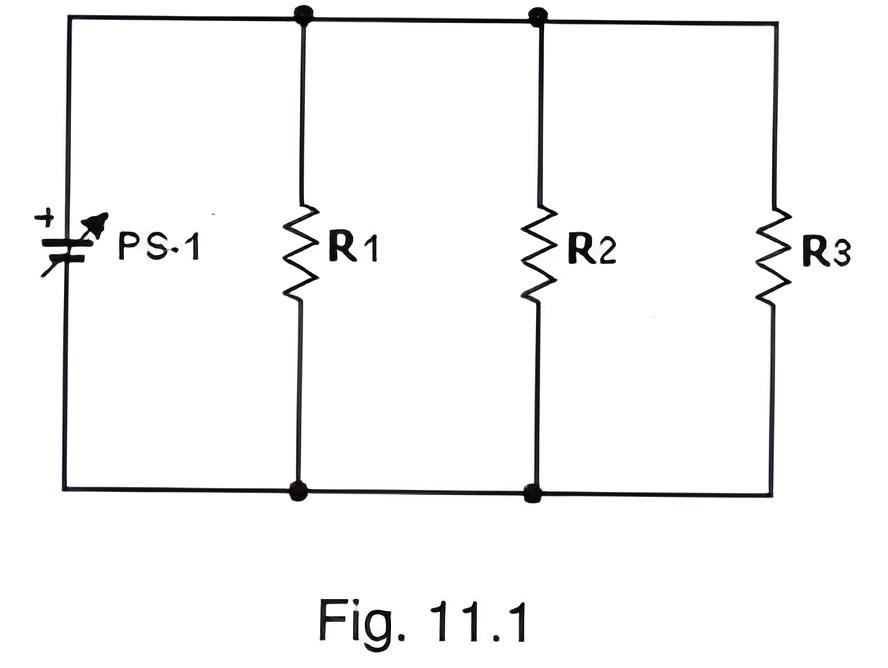
\includegraphics[scale=0.2]{imagenes/1}
	\end{figure}
	\\ Si PS-1 es igual a $6V R_{1}=6.8k,R_{2}=3.3k,R_{3}=1.2k la intensidad que la fuente proporciona es: 7.70mA$
\end{enumerate}
\section{Equipo}
El siguiente equipo es necesario para realizar el experimento 
\begin{enumerate}
	
	\item	Modulo experimental
 \item	DMM (multímetro digital)
	
\end{enumerate}
\section{Procedimiento}
\begin{enumerate}
	\item 	Efectué los cálculos para el circuito de la fig 1.2
\item	Lleve la salida de las fuentes a 0V. conecte el circuito
\item 	Lleve la salida de ps a 6V
\item Mida y anote las corrientes que circulan desde/hacia el nodo a través de $R_{1},R_{2}  y R_{3}$(dichas corrientes serán negativas)\\
Ahora mida y anote la corriente que ingresa en el nodo desde la fuente de alimentación. Esta corriente será considerada positiva
\item 	Para calcular la corriente total en el nodo, sume las cuatro corrientes algebraicamente (respetando sus signos)
La suma de las corrientes en el nodo $= (-0.88mA-1.82mA-5.00mA=-770mA)$
\item Lleve la salida de PS-1 a 0V. Estudie el circuito de la figura 11.3
\begin{figure}[h]
	\centering
	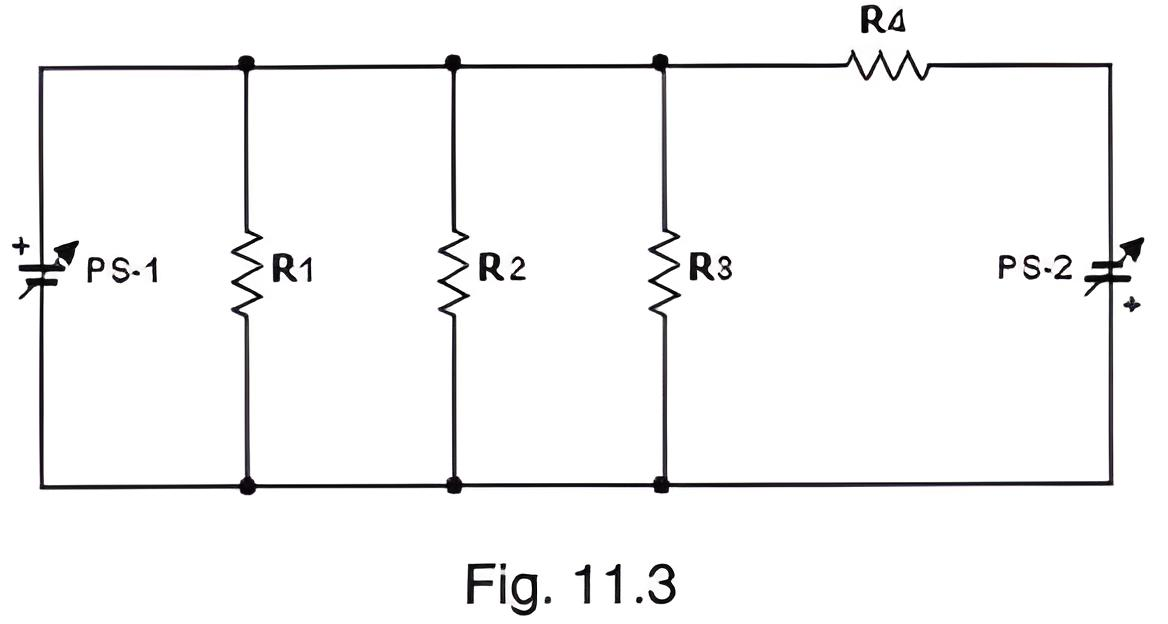
\includegraphics[scale=0.2]{imagenes/2}
\end{figure}
	\item 	Conecte el circuito como se indica en la figura 11.3
\item 	Fije la salida de PS-1 en 6V, y la salida de PS-2 en -3V
	\item 	Mida y anote la corriente que circula por$ R_{1},R_{2},R_{3} $y $ R_{4}$
	\item 	Para calcular la corriente total en el nodo, sume las cuatro corrientes algebraicamente (respetando sus signos).\\
	Suma de las corrientes en el nodo $= 0.88mA+1.82mA+5mA+2.05mA=9.75mA$
	
\end{enumerate}
\section{Autoevaluación}
\begin{enumerate}
	\item	La corriente total que sale de un nodo es: la suma total de las corrientes que entran al nodo.
	\item	La suma de las corrientes de un nodo es: igual a 0.
	\item 	Si en la figura 11.1 todas las resistencias son del mismo valor y la fuente de tensión PS-1 = 12 V la relación entre la corriente total que fluye por cada resistor es: proporcional al valor de la fuente de voltaje.
\end{enumerate}
\section{Conclusiones}
Cuando se conectan resistencias en paralelo, sus terminales están conectados de manera que ambos extremos de cada resistencia estén conectados al mismo par de nodos o puntos del circuito. 
Si las resistencias en paralelo tienen el mismo valor la intensidad es proporcional a la fuente de voltaje como se aprecia en la figura anterior.
\section{Anexo}
\begin{figure}[h]
	\centering
	\begin{minipage}{0.5\textwidth}
		\centering
		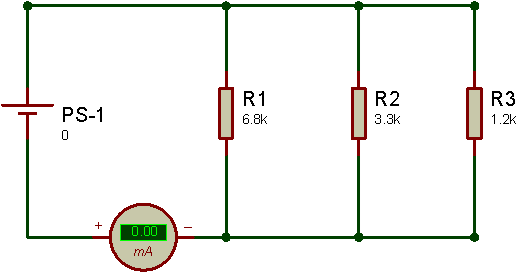
\includegraphics[width=0.8\linewidth]{imagenes/3}
	\end{minipage}%
	\begin{minipage}{0.5\textwidth}
		\centering
		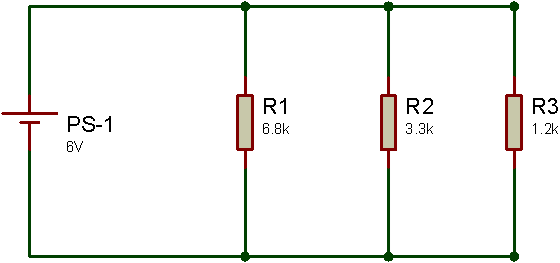
\includegraphics[width=0.8\linewidth]{imagenes/4}
	\end{minipage}
\end{figure}

\begin{figure}[h]
	\centering
	\begin{minipage}{0.5\textwidth}
		\centering
		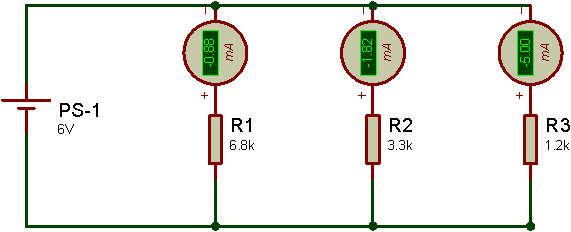
\includegraphics[width=0.8\linewidth]{imagenes/5}
	\end{minipage}%
	\begin{minipage}{0.5\textwidth}
		\centering
		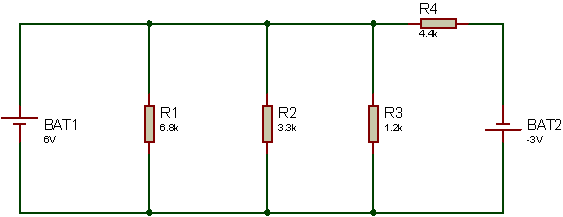
\includegraphics[width=0.8\linewidth]{imagenes/6}
	\end{minipage}
\end{figure}

\begin{figure}[h]
	\centering
	\begin{minipage}{0.5\textwidth}
		\centering
		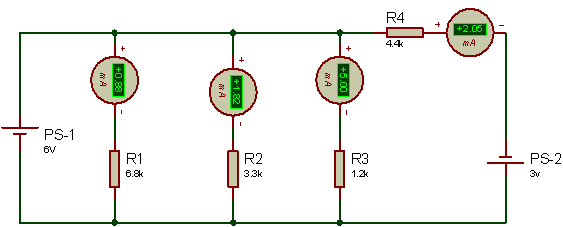
\includegraphics[width=0.8\linewidth]{imagenes/7}
	\end{minipage}%
	\begin{minipage}{0.5\textwidth}
		\centering
		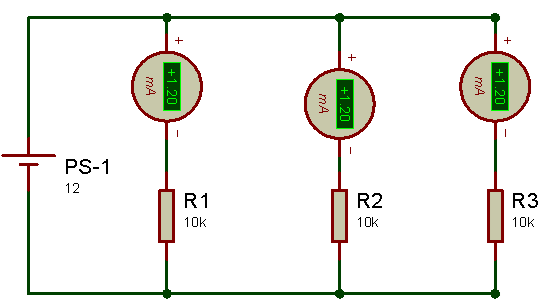
\includegraphics[width=0.8\linewidth]{imagenes/8}
	\end{minipage}
\end{figure}